\documentclass[10pt,letterpaper]{article}

% --- Soporte de Idioma y Codificación ---
\usepackage[utf8]{inputenc}       
\usepackage[T1]{fontenc}          
\usepackage[spanish]{babel} %puedo añadir despues de spanish esto para que diga tabla y no cuadro es-tabla
\addto\captionsspanish{\renewcommand{\abstractname}{Abstract}} %para que diga Abstract en vez de Resumen

% --- Símbolos Matemáticos Avanzados ---
\usepackage{amsmath}              
\usepackage{amsfonts}             
\usepackage{amssymb}              
\usepackage{amsthm}         

% --- Gráficas
\usepackage{graphicx}      
\usepackage[spanish,noabbrev]{cleveref} %para citar las graficas

% --- Tablas Mejoradas ---
\usepackage{booktabs}             
\usepackage{array}                
\usepackage{multirow}             

% --- Gestión de Márgenes ---
%\usepackage{fullpage}
%\usepackage[margin=2cm]{geometry}  %poniendole las margenes

% --- Gestión de Bibliografía con Natbib (Perfecto para tu BibTeX) ---
%\usepackage[numbers,sort&compress]{natbib} % Citas numéricas agrupadas automáticamente
\usepackage[authoryear,sort]{natbib}  %forma APA


% --- Datos del Documento ---
\title{Estudio de clasificación de uso excesivo de internet como un problema de adicción por medio de parámetros fácilmente medibles y voy a escribir mucho mas}
\author{Rafael Santiago Bedoya, Jose Ricardo Florez \\ Wilson Panesso, Angie Giselle Perez}
\date{}                     % Inserta de forma automática la fecha actual en español

% =========================================================================
\begin{document}

\maketitle                        % Genera el título automáticamente

\begin{abstract}
Este trabajo presenta el análisis del caso de uso excesivo del internet en niños y adolescentes como un caso de adicción, realizamos un recorrido sobre los posibles cambios comportamentales asociados tales como parámetros de aptitud física, rendimiento físico y patrones de sueño.Aal igual que factores de riesgo que pueden influir en la tendencia a caer en adicción. De esta forma este estudio busca proponer una clasificación preliminar basada en patrones \citep{garcia2008riesgos} fácilmente observables para aplicar de esta manera los estudios clínicos pertinentes para identificar la adicción.
\end{abstract}

\newpage
\tableofcontents

\newpage

\section{Introducción}
Aunque un articulo rara vez lleva tabla de contenido, lo incluiremos para visualizarlo en LaTex esta es mi introduccion y va a ser mucho mas larga

\section{Objetivos}

\begin{itemize}
\item Objetivo de encontrar las medidas
\item Objetivo 2
\item este es el nuevo objetivo que acabo de escribir

\end{itemize}

\subsection{Objetivos Especificos}
\begin{enumerate}
\item primer objetivo
    
\end{enumerate}


\newpage
\section{Estado del arte}
Esto es lo que tenemos que escribir, voy a citar los articulos para que me genere la bibliografia, solo van a aparecer en la bibliografia los articulos que fueron citados  \citep{lifestyle_changes, mobile_addiction, redes_sociales_gallegos, eficacia_academica, hurtado2024impactos}. Tambien añadire una tabla sin nada como referencia.

Vamos a poner simbolos extraños para ver el poder de LaTex: podemos incluir dentro el mismo texto $\alpha = \sum_{i=1}^n \Gamma X^2$ aqui continue aqui el texto.

\medskip   %puedo usar \bigskip si quiero mas espacio, o smallskip, aunque este no lo recomiendo
Ahora muestro la forma 2:
\[ \alpha = \sum_{i=1}^n \gamma X^2  \]

Finalmente la ultima forma es:
\begin{equation}
\alpha = \sum_{i=1}^n \gamma X^2
\label{eq_ejemplo}
\end{equation}

De esta manera puedo citar mi ecuacion, por ejemplo referenciando la ecuacion \eqref{eq_ejemplo} podemos ver....

Vamos con lo aprendido a escribir una funcion que seguramente aparecera en el modelo, la definicion de la clasificacion:

\bigskip
Sea $F$ una funcion definida de la siguiente manera:
\begin{equation}
F = 
\begin{cases} 
1, & \text{si se sospecha que el menor tiene una adicción al internet,} \\ 
0, & \text{en caso contrario} 
\end{cases}
\label{eq:funcion_binaria}
\end{equation}


\begin{table}[h]
\centering
\begin{tabular}{ccc}  %la cantidad de c, es la cantidad de columnas, 4 columnas seria cccc
\hline %añade linea horizontal
\textbf{Columna 1} & \textbf{Columna 2} & \textbf{Columna 3} \\
\hline
Dato A & Ecuación $x^2$ & Texto 1 \\  %agregar cada fila, separada por el simbolo &
Dato B & Símbolo $\beta$ & Texto 2 \\
\hline
\end{tabular}
\end{table}

Finalmente vamos a agregar una imagen, para ello la imagen debe estar en la misma carpeta de nuestro archivo .tex, y se agrega de forma muy sencilla.

\begin{figure}[htbp] %here top bottom  page, este es el orden de prioridades para que el grafico quede lo mas cercano posible a donde yo lo quiero, p es que si el grafico es demasiado grande, el lo manda a una pagina dedicada a graficos.
\centering
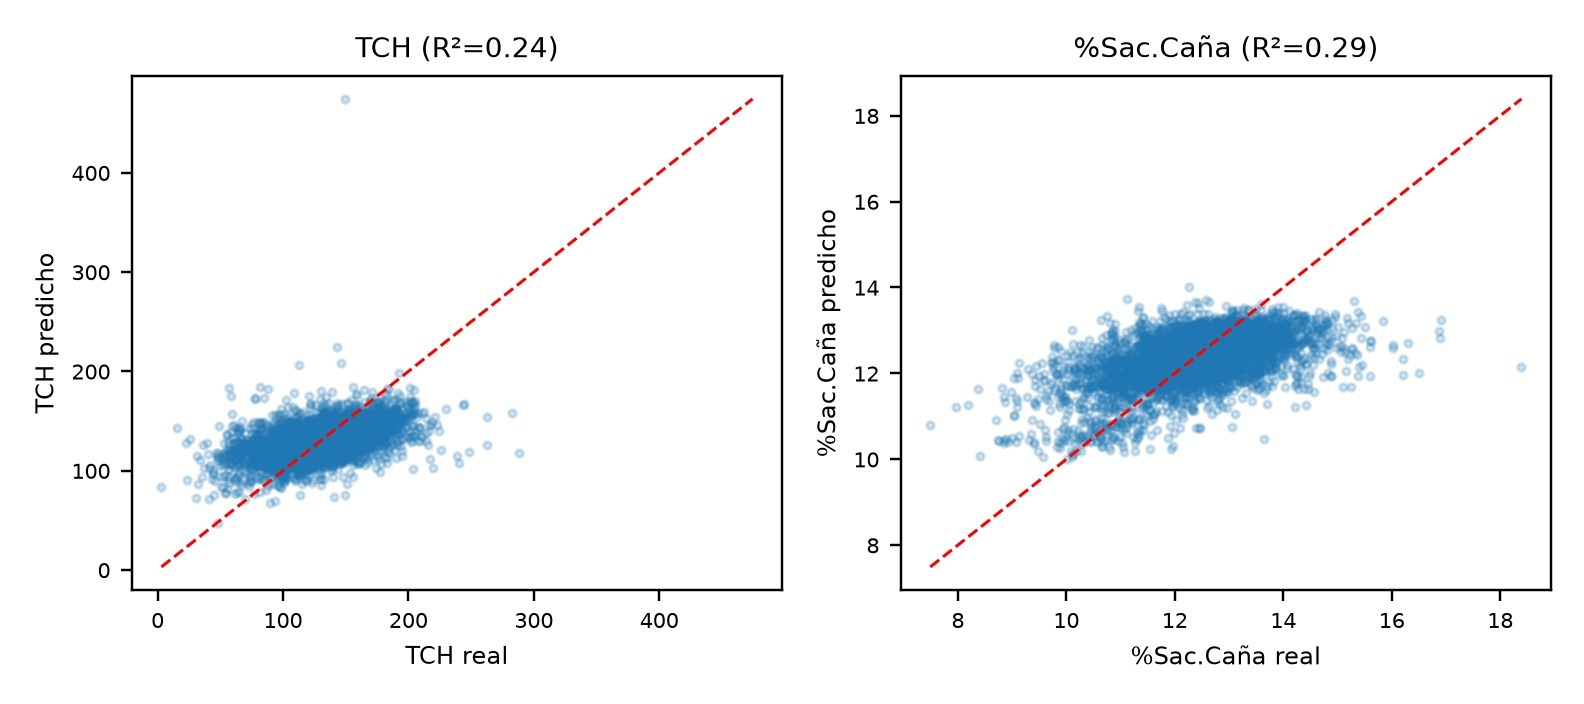
\includegraphics[width=0.6\textwidth]{WhatsApp Image 2026-10-07 at 8.54.12 PM.jpeg }
\caption{Regresión Logística Regularizada}
\label{fig_reg_logistica}
\end{figure}


Igualmente puedo citar mi imagen, teniendo en cuenta la imagen \cref {fig_reg_logistica} podemos observar que realmente el modelo lineal no modelo de forma apropiada la naturaleza de los datos.
\newpage
\bibliographystyle{apalike} %arma la bibliografia en forma APA
%\bibliographystyle{unsrtnat} % Ordena las referencias por aparición (1, 2, 3...)
\bibliography{archivo_bibtex} 

\end{document}